\documentclass[border=8mm]{standalone}
\usepackage{tikz}
\usepackage{xcolor}

\begin{document}
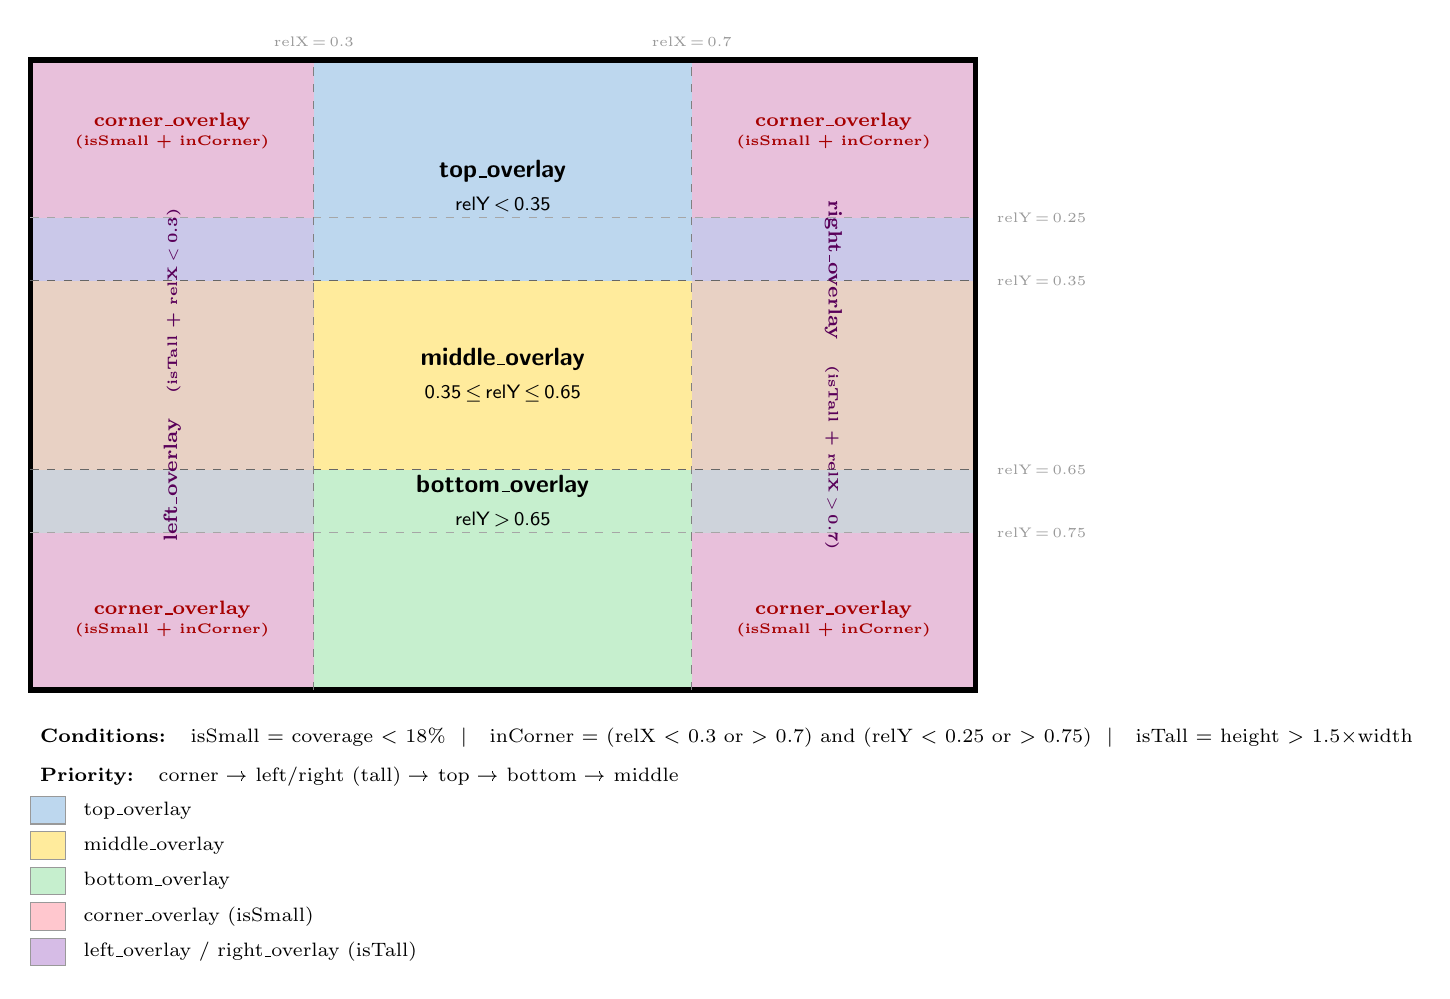
\begin{tikzpicture}[font=\sffamily\small]

% Viewport: 12 × 8 units.  Y axis is flipped so relY=0 is at the top.
%   y = 8 × (1 − relY)
%   relY=0.25 -> y=6.0,   relY=0.35 -> y=5.2
%   relY=0.65 -> y=2.8,   relY=0.75 -> y=2.0
%   relX=0.30 -> x=3.6,   relX=0.70 -> x=8.4

% ── Region fills ─────────────────────────────────────────────────────────────
\definecolor{Ctop}{RGB}{189,215,238}   % blue  – top_overlay
\definecolor{Cmid}{RGB}{255,235,156}   % amber – middle_overlay
\definecolor{Cbot}{RGB}{198,239,206}   % green – bottom_overlay
\definecolor{Ccor}{RGB}{255,199,206}   % pink  – corner_overlay
\definecolor{Csid}{RGB}{214,188,230}   % lilac – left/right_overlay

% Horizontal bands (back layer)
\fill[Ctop] (0,5.2) rectangle (12,8);
\fill[Cmid] (0,2.8) rectangle (12,5.2);
\fill[Cbot] (0,0)   rectangle (12,2.8);

% Corner zones (overlay top/bottom bands)
\fill[Ccor] (0,6)   rectangle (3.6,8);
\fill[Ccor] (8.4,6) rectangle (12,8);
\fill[Ccor] (0,0)   rectangle (3.6,2);
\fill[Ccor] (8.4,0) rectangle (12,2);

% Side strips (semi-transparent — tall elements override top/middle/bottom)
\fill[Csid,opacity=0.55] (0,0)   rectangle (3.6,8);
\fill[Csid,opacity=0.55] (8.4,0) rectangle (12,8);

% ── Viewport border ───────────────────────────────────────────────────────────
\draw[line width=2pt] (0,0) rectangle (12,8);

% ── Grid lines ───────────────────────────────────────────────────────────────
% Corner-zone boundaries (relY = 0.25 / 0.75)
\draw[dashed,black!35,thin] (0,6)   -- (12,6);
\draw[dashed,black!35,thin] (0,2)   -- (12,2);
% Band boundaries (relY = 0.35 / 0.65)
\draw[dashed,black!60]      (0,5.2) -- (12,5.2);
\draw[dashed,black!60]      (0,2.8) -- (12,2.8);
% Vertical zone boundaries (relX = 0.30 / 0.70)
\draw[dashed,black!50]      (3.6,0) -- (3.6,8);
\draw[dashed,black!50]      (8.4,0) -- (8.4,8);

% ── Threshold annotations (outside viewport) ──────────────────────────────────
\foreach \y/\lbl in {6.0/0.25, 5.2/0.35, 2.8/0.65, 2.0/0.75}
  \node[right,black!40,font=\tiny] at (12.15,\y) {relY\,=\,\lbl};

\node[above,black!40,font=\tiny] at (3.6,8.05) {relX\,=\,0.3};
\node[above,black!40,font=\tiny] at (8.4,8.05) {relX\,=\,0.7};

% ── Region labels ─────────────────────────────────────────────────────────────

% top_overlay — in the central column of the top band
\node[align=center] at (6,6.4)
  {\textbf{top\_overlay}\\[1pt]\scriptsize relY\,$<$\,0.35};

% middle_overlay
\node[align=center] at (6,4.0)
  {\textbf{middle\_overlay}\\[1pt]\scriptsize 0.35\,$\leq$\,relY\,$\leq$\,0.65};

% bottom_overlay
\node[align=center] at (6,2.4)
  {\textbf{bottom\_overlay}\\[1pt]\scriptsize relY\,$>$\,0.65};

% corner_overlay × 4  (small element + corner zone)
\foreach \x/\y in {1.8/7.1, 10.2/7.1, 1.8/0.9, 10.2/0.9}
  \node[align=center,font=\scriptsize\bfseries,text=red!65!black] at (\x,\y)
    {corner\_overlay\\[-1pt]\tiny(isSmall + inCorner)};

% left_overlay / right_overlay (tall elements — rotated labels along sides)
\node[rotate=90,align=center,font=\scriptsize\bfseries,text=violet!70!black]
  at (1.8,4.0) {left\_overlay\quad\tiny(isTall + relX\,$<$\,0.3)};
\node[rotate=-90,align=center,font=\scriptsize\bfseries,text=violet!70!black]
  at (10.2,4.0) {right\_overlay\quad\tiny(isTall + relX\,$>$\,0.7)};

% ── Condition summary (below viewport) ────────────────────────────────────────
\node[anchor=north west,align=left,font=\scriptsize] at (0,-0.35) {%
  \textbf{Conditions:}~~
  isSmall = coverage $<$ 18\%~~$|$~~
  inCorner = (relX $<$ 0.3 or $>$ 0.7) and (relY $<$ 0.25 or $>$ 0.75)~~$|$~~
  isTall = height $>$ 1.5$\times$width};

\node[anchor=north west,align=left,font=\scriptsize] at (0,-0.85) {%
  \textbf{Priority:}~~
  corner \textrightarrow{} left/right (tall) \textrightarrow{} top \textrightarrow{}
  bottom \textrightarrow{} middle};

% ── Legend ────────────────────────────────────────────────────────────────────
\begin{scope}[shift={(0,-1.7)}, font=\scriptsize]
  \foreach \col/\lbl/\yi in {
      Ctop/top\_overlay/0,
      Cmid/middle\_overlay/-0.45,
      Cbot/bottom\_overlay/-0.9,
      Ccor/{corner\_overlay (isSmall)}/-1.35,
      Csid/{left\_overlay / right\_overlay (isTall)}/-1.8}
    {
      \fill[\col] (0,\yi) rectangle (0.45,\yi+0.35);
      \draw[black!40,thin] (0,\yi) rectangle (0.45,\yi+0.35);
      \node[right] at (0.55,\yi+0.175) {\lbl};
    }
\end{scope}

\end{tikzpicture}
\end{document}
